%%%%%%%%%%%%%%%%%%%%%%%%%%%%%%%% ARITHMETIC OPS

\lecture{Operações aritméticas}{arith}

\section{\insertlecture}

\subsection{Representação de inteiros}

\begin{frame}
  \frametitle{Representação de inteiros}

Um {\em byte} pode representar os numeros de 0 a 255 da seguinte forma,\\
\begin{center}
    \begin{tabular}{lll}
      00000000 & = & 0 \\
      00000001 & = & 1 \\
      00101001 & = & 41 \\
      10000000 & = & 128 \\
      11111111 & = & 255 \\
    \end{tabular}
  \end{center}
  
\pause
 Um valor inteiro $A$ de uma sequência de n bits de dígitos binários
 $a_{n-1}a_{n-2}\ldots a_1a_0$ pode ser obtido pela seguinte fórmula:
 \begin{equation}
   \label{eq:magnitudesinal}
   A = \sum_{i=0}^{n-1}2^ia_i
 \end{equation}

\end{frame}

\def\thetitle{Representação em sinal-magnitude}

\subsection{\thetitle}

\begin{frame}[fragile]{\thetitle}

O bit mais significativo (mais à esquerda) representa o \alert{sinal} e o
restante, a \alert{magnitude}.

\begin{center}  
  \begin{tabular}{lll}
    +18 & = & 00010010 \\
    \alert{--}18 & = & \alert{1}0010010 (sinal-magnitude)\\
  \end{tabular}
\end{center}  

O valor do inteiro $A$ é calculado da seguinte forma:\\

\pause
\begin{equation}
  \label{eq:sinalmagnitudemenos}
  A = 
  \begin{cases}
     \displaystyle\sum_{i=0}^{n-1}2^ia_i & \text{se}\ a_{n-1}=0\\
    -\displaystyle\sum_{i=0}^{n-1}2^ia_i & \text{if}\ a_{n-1}=1
   \end{cases}
\end{equation}

\end{frame}

\def\thetitle{Representação em complemento de dois}

\subsection{\thetitle}

\begin{frame}{\thetitle}
\begin{center}
  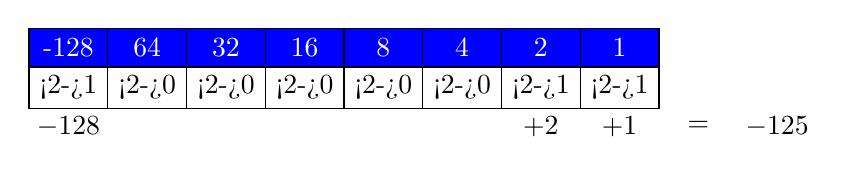
\begin{tikzpicture}
    \tikzset{cell/.style={minimum width=1cm,minimum height=0.5cm,rectangle,draw}}
    \foreach \x/\m/\bin in {0/-128/1,1/64/0,2/32/0,3/16/0,4/8/0,5/4/0,6/2/1,7/1/1} {
      \node[cell,fill=blue,font=\color{white}] at (\x,0) {\m};
      \node[cell] at (\x,-.5) {\only<2->{\bin}};
    }
    \node<3-> at (0,-1) {$-128$};
    \node<3-> at (6,-1) {$+2$};    
    \node<3-> (less) at (7,-1) {$+1$};
    \node<3-> (eq) [right of=less] {$=$};
    \node<3-> [right of=eq] {$-125$};
  \end{tikzpicture}
\end{center}

\only<4>{
\begin{equation}
  \label{eq:sinalmagnitudemenos}
  A = -2^{n-1}a_{n-1} + \displaystyle\sum_{i=0}^{n-2}2^ia_i
\end{equation}
}

\end{frame}


\def\thetitle{Aritmética com inteiros}

\subsection{\thetitle}

\frame{\author{}\date{}\institute{}\title{\thetitle}\titlepage}

\begin{frame}{Negação}{Complemento de dois}

  \begin{tabbing}
    $\alert{+}18$  $\rightarrow$ \hspace{3cm} \= $00010010$ \\
    {\small complemento bit a bit}  $\rightarrow$ \> $111011$\=$01$ \\
      \>$+$ \> $1$ \\
       \> $\overline{11101110}$ $=-18$\\
  \end{tabbing}

\pause
  \begin{tabbing}
    $\alert{-}18$  $\rightarrow$ \hspace{3cm}  \= $111011$\=$10$ \\
    {\small complemento bit a bit} $\rightarrow$ \> $00010001$ \\
    \>$+$ \> $1$ \\
    \> $\overline{00010010}$ $=+18$\\
  \end{tabbing}

\end{frame}

\subsubsection{Adição}

\begin{frame}{Adição}{Complemento de dois}

\begin{columns}
\begin{column}{.3\textwidth}
  \begin{tabular}{rcl}
      $1001$ & = & $-7$ \\
      $+\ 0101$ & = & $5$ \\\hline
      $1110$ & = & $-2$ \\
     \end{tabular}
   \end{column}

\begin{column}{.3\textwidth}
  \begin{tabular}{rcl}
      $1100$ & = & $-4$ \\
      $+\ 0100$ & = & $4$ \\\hline
      ${\color{gray}1}0000$ & = & $0$ \\
     \end{tabular}
   \end{column}
 \end{columns}

\pause
\bigskip
{\color{gray}\hrule}
\bigskip
\begin{columns}
\begin{column}{.3\textwidth}
  \begin{tabular}{rcl}
      $0011$ & = & $3$ \\
      $+\ 0100$ & = & $4$ \\\hline
      $0111$ & = & $7$ \\
     \end{tabular}
   \end{column}

\begin{column}{.3\textwidth}
  \begin{tabular}{rcl}
      $1100$ & = & $-4$ \\
      $+\ 1111$ & = & $-1$ \\\hline
      ${\color{gray}1}1011$ & = & $-5$ \\
     \end{tabular}
   \end{column}

\end{columns}

\pause
\bigskip
{\color{gray}\hrule}
\bigskip
\begin{columns}
\begin{column}{.3\textwidth}
  \begin{tabular}{rcl}
      $\alert{0}101$ & = & $5$ \\
      $+\ \alert{0}100$ & = & $4$ \\\hline
      $\alert{1}001$ & = & \alert{\tt Overflow} \\
     \end{tabular}
   \end{column}

\begin{column}{.3\textwidth}
  \begin{tabular}{rcl}
      $\alert{1}001$ & = & $-7$ \\
      $+\ \alert{1}010$ & = & $-6$ \\\hline
      $\alert{0}011$ & = & \alert{\tt Overflow} \\
     \end{tabular}
   \end{column}


\end{columns}


\end{frame}

\def\thetitle{Subtração}

\subsubsection{\thetitle}

\begin{frame}{\thetitle}
\begin{center}
  \begin{tikzpicture}
    \tikzset{cell/.style={minimum width=1cm,minimum height=0.5cm}}
    \foreach \x/\s/\m/\c/\r/\rf in {0/0/0/1/0/0,1/1/0/1/0/0,2/0/1/0/1/1,3/1/0/1/0/1} {
      \node[cell] at (\x,0) {\s};
      \node[cell] at (\x,-.5) {\only<1>{\m}\only<2->{\color{red}\c}};
      \node[cell] at (\x,-1.5) {\only<3->{\r}};
      \node[cell] at (\x,-3) {\only<5>{\rf}};
    }
    \node at (4,0) {$\equiv\ 5$};
    \node<1> at (6,0) {\small subtraendo};
    \node<1> at (3.80,-.5) {$\equiv$};
    \node (two) at (4.25,-.5) {$2$};
    \node<1> at (6,-.5) {\small minuendo};
    \node at (-.5,-.5) {\only<1>{$-$}\only<2->{\color{red}$+$}};
    \node<2-> [right of=two,anchor=west] {\small \color{red}
      complemento bit a bit};
    \draw (-.5,-1) -- (3.5,-1);
    \node at (-1,-1.5) {\only<3>{$1$}};
    \node<4-> at (3,-2) {$1$};
    \node<4-> at (-.5,-2) {$+$};
    \draw<4-> (-.5,-2.5) -- (3.5,-2.5);
    \node<5> at (4,-3) {$\equiv\ 3$};
  \end{tikzpicture}
\end{center}

\end{frame}


\def\thetitle{Multiplicação}
\subsubsection{\thetitle}

\begin{frame}{\thetitle}
\begin{center}
  \begin{tikzpicture}
    \tikzset{cell/.style={minimum width=1cm,minimum height=0.5cm}}
    \foreach \x/\s/\m/\c/\pa/\pb in {0/0/{\color<5>{red}0}/0/0/0,1/1/{\color<4>{red}0}/0/0/1,2/0/{\color<3>{red}1}/1/0/0,3/1/{\color<2>{red}0}/0/0/1} {
      \node[cell] at (\x,0) {\s};
      \node[cell] at (\x,-.5) {\m};
      \node<2->[cell] at (\x,-1.5) {\pa};
      \node<3->[cell] at (\x-1,-2) {\pb};
      \node<4->[cell] at (\x-2,-2.5) {\pa};
      \node<5->[cell] at (\x-3,-3) {\pa};
      \node<6->[cell] at (\x-1,-4) {\pb};
    }
    \node at (4,0) {$\equiv\ 5$};
    \node<1> at (6,0) {\small multiplicando};
    \node at (4,-.5) {$\equiv\ 2$};
    \node<1> at (6,-.5) {\small multiplicador};
    \node at (-.5,-.5) {$\times$};
    \draw (-3.5,-1) -- (3.5,-1);
    \node<6-> at (-3.5,-3) {$+$};
    \draw<5-> (-3.5,-3.5) -- (3.5,-3.5);
    \foreach \x in {4,-1,-2} {
      \node<6->[cell] at (\x-1,-4) {$0$};
    }
    \node<6> at (4,-4) {$\equiv\ 10$};
  \end{tikzpicture}
\end{center}

\end{frame}

\begin{frame}{Exercícios}
  \begin{enumerate}
  \item Represente os seguintes valores de complemento de 2 em
    decimal: 
    \begin{itemize}
      \item 1101011
      \item 0101101
      \end{itemize}
    \item Suponha que os números sejam representados por complemento de
    2 com 8 bits. Mostre os seguintes cálculos:
    \begin{itemize}
    \item $6+13$
    \item $5+4$
    \end{itemize}
  \item Realize as seguintes subtrações utilizando 4 bits: 
    \begin{itemize}
      \item $8-4$
      \item $9-2$
      \end{itemize}
    \item Realize as seguintes multiplicações: 
      \begin{itemize}
      \item $3\times 4$
      \item $2 \times 3$
      \end{itemize}
    \end{enumerate}
  

\end{frame}

\begin{frame}{Tabela de conversão decimal, hexadecimal, octal, binário.}
\small

\begin{columns}
  \begin{column}{.5\textwidth}
    
    \begin{tabular}{cccc}\hline
      \bf Dec& 	\bf Hex& 	\bf Oct &	\bf Bin \\\hline
      000&	00&	000&	00000000\\
      001&	01&	001&	00000001\\
      002&	02&	002&	00000010\\
      003&	03&	003&	00000011\\
      004&	04&	004&	00000100\\
      005&	05&	005&	00000101\\
      006&	06&	006&	00000110\\
      007&	07&	007&	00000111\\
      008&	08&	010&	00001000\\
      009&	09&	011&	00001001\\
      010&	0A&	012&	00001010\\
      011&	0B&	013&	00001011\\
      012&	0C&	014&	00001100\\
      013&	0D&	015&	00001101\\
      014&	0E&	016&	00001110\\
      015&	0F&	017&	00001111\\\hline
    \end{tabular}

  \end{column}

  \begin{column}{.5\textwidth}
    \begin{tabular}{cccc}\hline
      \bf Dec& \bf 	Hex &\bf	Oct &\bf	Bin\\\hline
      016&	10&	020&	00010000\\
      017&	11&	021&	00010001\\
      018&	12&	022&	00010010\\
      019&	13&	023&	00010011\\
      020&	14&	024&	00010100\\
      021&	15&	025&	00010101\\
      022&	16&	026&	00010110\\
      023&	17&	027&	00010111\\
      024&	18&	030&	00011000\\
      025&	19&	031&	00011001\\
      026&	1A&	032&	00011010\\
      027&	1B&	033&	00011011\\
      028&	1C&	034&	00011100\\
      029&	1D&	035&	00011101\\
      030&	1E&	036&	00011110\\
      031&	1F&	037&	00011111\\\hline
    \end{tabular}
  \end{column}
\end{columns}
\end{frame}
